\documentclass[11pt,a4paper,]{article}
\usepackage{lmodern}

\usepackage{amssymb,amsmath}
\usepackage{ifxetex,ifluatex}
\usepackage{fixltx2e} % provides \textsubscript
\ifnum 0\ifxetex 1\fi\ifluatex 1\fi=0 % if pdftex
  \usepackage[T1]{fontenc}
  \usepackage[utf8]{inputenc}
\else % if luatex or xelatex
  \usepackage{unicode-math}
  \defaultfontfeatures{Ligatures=TeX,Scale=MatchLowercase}
\fi
% use upquote if available, for straight quotes in verbatim environments
\IfFileExists{upquote.sty}{\usepackage{upquote}}{}
% use microtype if available
\IfFileExists{microtype.sty}{%
\usepackage[]{microtype}
\UseMicrotypeSet[protrusion]{basicmath} % disable protrusion for tt fonts
}{}
\PassOptionsToPackage{hyphens}{url} % url is loaded by hyperref
\usepackage[unicode=true]{hyperref}
\hypersetup{
            pdftitle={Sectoral Employment Dynamics in Australia},
            pdfborder={0 0 0},
            breaklinks=true}
\urlstyle{same}  % don't use monospace font for urls
\usepackage{geometry}
\geometry{a4paper, centering, text={16cm,25cm}}
\usepackage[style=apa,]{biblatex}
\addbibresource{references.bib}
\usepackage{longtable,booktabs}
% Fix footnotes in tables (requires footnote package)
\IfFileExists{footnote.sty}{\usepackage{footnote}\makesavenoteenv{long table}}{}
\IfFileExists{parskip.sty}{%
\usepackage{parskip}
}{% else
\setlength{\parindent}{0pt}
\setlength{\parskip}{6pt plus 2pt minus 1pt}
}
\setlength{\emergencystretch}{3em}  % prevent overfull lines
\providecommand{\tightlist}{%
  \setlength{\itemsep}{0pt}\setlength{\parskip}{0pt}}
\setcounter{secnumdepth}{5}

% set default figure placement to htbp
\makeatletter
\def\fps@figure{htbp}
\makeatother


\title{Sectoral Employment Dynamics in Australia}

%% MONASH STUFF

%% CAPTIONS
\RequirePackage{caption}
\DeclareCaptionStyle{italic}[justification=centering]
 {labelfont={bf},textfont={it},labelsep=colon}
\captionsetup[figure]{style=italic,format=hang,singlelinecheck=true}
\captionsetup[table]{style=italic,format=hang,singlelinecheck=true}


%% FONT
\RequirePackage{bera}
\RequirePackage[charter,expert,sfscaled]{mathdesign}
\RequirePackage{fontawesome}

%% HEADERS AND FOOTERS
\RequirePackage{fancyhdr}
\pagestyle{fancy}
\rfoot{\Large\sffamily\raisebox{-0.1cm}{\textbf{\thepage}}}
\makeatletter
\lhead{\textsf{\expandafter{\@title}}}
\makeatother
\rhead{}
\cfoot{}
\setlength{\headheight}{15pt}
\renewcommand{\headrulewidth}{0.4pt}
\renewcommand{\footrulewidth}{0.4pt}
\fancypagestyle{plain}{%
\fancyhf{} % clear all header and footer fields
\fancyfoot[C]{\sffamily\thepage} % except the center
\renewcommand{\headrulewidth}{0pt}
\renewcommand{\footrulewidth}{0pt}}

%% MATHS
\RequirePackage{bm,amsmath}
\allowdisplaybreaks

%% GRAPHICS
\RequirePackage{graphicx}
\setcounter{topnumber}{2}
\setcounter{bottomnumber}{2}
\setcounter{totalnumber}{4}
\renewcommand{\topfraction}{0.85}
\renewcommand{\bottomfraction}{0.85}
\renewcommand{\textfraction}{0.15}
\renewcommand{\floatpagefraction}{0.8}


%\RequirePackage[section]{placeins}

%% SECTION TITLES


%% SECTION TITLES
\RequirePackage[compact,sf,bf]{titlesec}
\titleformat*{\section}{\Large\sf\bfseries\color[rgb]{0.7,0,0}}
\titleformat*{\subsection}{\large\sf\bfseries\color[rgb]{0.7,0,0}}
\titleformat*{\subsubsection}{\sf\bfseries\color[rgb]{0.7,0,0}}
\titlespacing{\section}{0pt}{2ex}{.5ex}
\titlespacing{\subsection}{0pt}{1.5ex}{0ex}
\titlespacing{\subsubsection}{0pt}{.5ex}{0ex}


%% TITLE PAGE
\def\Date{\number\day}
\def\Month{\ifcase\month\or
 January\or February\or March\or April\or May\or June\or
 July\or August\or September\or October\or November\or December\fi}
\def\Year{\number\year}

%% LINE AND PAGE BREAKING
\sloppy
\clubpenalty = 10000
\widowpenalty = 10000
\brokenpenalty = 10000
\RequirePackage{microtype}

%% PARAGRAPH BREAKS
\setlength{\parskip}{1.4ex}
\setlength{\parindent}{0em}

%% HYPERLINKS
\RequirePackage{xcolor} % Needed for links
\definecolor{darkblue}{rgb}{0,0,.6}
\RequirePackage{url}

\makeatletter
\@ifpackageloaded{hyperref}{}{\RequirePackage{hyperref}}
\makeatother
\hypersetup{
     citecolor=0 0 0,
     breaklinks=true,
     bookmarksopen=true,
     bookmarksnumbered=true,
     linkcolor=darkblue,
     urlcolor=blue,
     citecolor=darkblue,
     colorlinks=true}

\usepackage[showonlyrefs]{mathtools}
\usepackage[no-weekday]{eukdate}

%% BIBLIOGRAPHY

\makeatletter
\@ifpackageloaded{biblatex}{}{\usepackage[style=authoryear-comp, backend=biber, natbib=true]{biblatex}}
\makeatother
\ExecuteBibliographyOptions{bibencoding=utf8,minnames=1,maxnames=3, maxbibnames=99,dashed=false,terseinits=true,giveninits=true,uniquename=false,uniquelist=false,doi=false, isbn=false,url=true,sortcites=false}

\DeclareFieldFormat{url}{\texttt{\url{#1}}}
\DeclareFieldFormat[article]{pages}{#1}
\DeclareFieldFormat[inproceedings]{pages}{\lowercase{pp.}#1}
\DeclareFieldFormat[incollection]{pages}{\lowercase{pp.}#1}
\DeclareFieldFormat[article]{volume}{\mkbibbold{#1}}
\DeclareFieldFormat[article]{number}{\mkbibparens{#1}}
\DeclareFieldFormat[article]{title}{\MakeCapital{#1}}
\DeclareFieldFormat[article]{url}{}
%\DeclareFieldFormat[book]{url}{}
%\DeclareFieldFormat[inbook]{url}{}
%\DeclareFieldFormat[incollection]{url}{}
%\DeclareFieldFormat[inproceedings]{url}{}
\DeclareFieldFormat[inproceedings]{title}{#1}
\DeclareFieldFormat{shorthandwidth}{#1}
%\DeclareFieldFormat{extrayear}{}
% No dot before number of articles
\usepackage{xpatch}
\xpatchbibmacro{volume+number+eid}{\setunit*{\adddot}}{}{}{}
% Remove In: for an article.
\renewbibmacro{in:}{%
  \ifentrytype{article}{}{%
  \printtext{\bibstring{in}\intitlepunct}}}

\AtEveryBibitem{\clearfield{month}}
\AtEveryCitekey{\clearfield{month}}

\makeatletter
\DeclareDelimFormat[cbx@textcite]{nameyeardelim}{\addspace}
\makeatother

\author{\sf{\Large\textbf{(Elvis) Zhixiang Yang}\\\large EBS Honours Student\\[0.5cm]}}

\date{\sf\Date~\Month~\Year}
\makeatletter
\lfoot{\sf Yang: \@date}
\makeatother


%%%% PAGE STYLE FOR FRONT PAGE OF REPORTS

\makeatletter
\def\organization#1{\gdef\@organization{#1}}
\def\telephone#1{\gdef\@telephone{#1}}
\def\email#1{\gdef\@email{#1}}
\makeatother
  \organization{Honours \textbf{Research Plan}, supervised by \textbf{Farshid Vahid}}

  \def\name{Department of\newline Econometrics \&\newline Business Statistics}

  \telephone{(03) 9905 2478}

  \email{BusEco-Econometrics@monash.edu}

\def\webaddress{\url{http://buseco.monash.edu/ebs/consulting/}}
\def\abn{12 377 614 012}
\def\extraspace{\vspace*{1.6cm}}
\makeatletter
\def\contactdetails{\faicon{phone} & \@telephone \\
                    \faicon{envelope} & \@email}
\makeatother

\usepackage[absolute,overlay]{textpos}
\setlength{\TPHorizModule}{1cm}
\setlength{\TPVertModule}{1cm}

%%%% FRONT PAGE OF REPORTS

\def\reporttype{Report for}

\long\def\front#1#2#3{
\newpage
\begin{textblock}{7}(12.7,28.2)\hfill
\includegraphics[height=0.6cm]{AACSB}~~~
\includegraphics[height=0.6cm]{EQUIS}~~~
\includegraphics[height=0.6cm]{AMBA}
\end{textblock}
\begin{singlespacing}
\thispagestyle{empty}
\vspace*{-1.4cm}
\hspace*{-1.4cm}
\hbox to 16cm{
  \hbox to 6.5cm{\vbox to 14cm{\vbox to 25cm{
    \includegraphics[width=6cm]{monash2}
    \vfill
    \includegraphics[width=3.5cm]{MBSportrait}
    \vspace{0.4cm}
    \par
    \parbox{6.3cm}{\raggedright
      \sf\color[rgb]{0.00,0.00,0.70}
      {\large\textbf{\name}}\par
      \vspace{.7cm}
      \tabcolsep=0.12cm\sf\small
      \begin{tabular}{@{}ll@{}}\contactdetails
      \end{tabular}
      \vspace*{0.3cm}\par
      ABN: \abn\par
    }
  }\vss}\hss}
  \hspace*{0.2cm}
  \hbox to 1cm{\vbox to 14cm{\rule{1pt}{26.8cm}\vss}\hss\hfill}
  \hbox to 10cm{\vbox to 14cm{\vbox to 25cm{
      \vspace*{3cm}\sf\raggedright
      \parbox{11cm}{\sf\raggedright\baselineskip=1.2cm
         \fontsize{24.88}{30}\color[rgb]{0.70,0.00,0.00}\sf\textbf{#1}}
      \par
      \vfill
      \large
      \vbox{\parskip=0.8cm #2}\par
      \vspace*{2cm}\par
      \reporttype\\[0.3cm]
      \hbox{#3}%\\[2cm]\
      \vspace*{1cm}
      {\large\sf\textbf{\Date~\Month~\Year}}
   }\vss}
  }}
\end{singlespacing}
\newpage
}

\makeatletter
\def\titlepage{\front{\expandafter{\@title}}{\@author}{\@organization}}
\makeatother

\usepackage{setspace}
\setstretch{1.5}

%% Any special functions or other packages can be loaded here.


\begin{document}
\titlepage

\graphicspath{ {/Users/elvisyang/Desktop/Sectoral Employment Forecsating /Research_Proporsal/elvis_plan/figure} }

\hypertarget{introduction}{%
\section{Introduction}\label{introduction}}

The COVID-19 pandemic has had a massive effect on economies around the world. Across different countries, millions of workers were furloughed or even lost their jobs as businesses struggled to survive \autocite{ny2020}. Same situation happened in Australia, due to more restrictions, many businesses closed their doors, while employees were working with less hours or being dismissed by companies. As a result of the continuous ``lockdown'' periods in 2020, the estimates made by the Australian Bureau of Statistics \autocite{ABS2021} concluded that 72\% of business generated less revenue and the underemployment rate hit historically high with 13.8\% by the end of April, 2020, only one month after the COVID-19 outbreak.

Our research is motivated by the lack of quantitative research on the employment of sub-sectors in Australia, as many studies have focused on the aggregated employment rate. A general problem of aggregated researches is the loss of hierarchical information, which may result in a biased conclusion or ``a illusion of employment prosperity''. Thus, a quantitative analysis of the sectoral employment and will overcome this problem, giving us a better scope to evaluate the impact of COVID-19 in Australia.

\hypertarget{research-aim-and-questions}{%
\section{Research aim and questions}\label{research-aim-and-questions}}

This research will extend \textcite{anderson2020} by using data on 87 sub-sectors, instead of 19 they used. I will develop a model for the sub-sectors to evaluate the long run effect and the COVID-19 post-impacts. I will also provide an contrafactual analysis based on the assumption ``if there is no pandemic''. subsectoral data will provide us more information, which will assist in getting a better employment dynamics understanding of Australia.

The overall research aim is to provide estimates of subsectoral employment based on historical data. Specifically, my goals are:

\begin{enumerate}
\def\labelenumi{\arabic{enumi}.}
\item
  To build up a time series model of employment in 87 sectors of the Australian economy
\item
  To use this model to conduct our contrafactual analysis.
\item
  To use this model to determine which sectors ave the highest impact on employment growth in the long run.
\end{enumerate}

\newpage

\hypertarget{review-of-literature}{%
\section{Review of literature}\label{review-of-literature}}

Our review of literature mainly focuses on two areas:

\begin{enumerate}
\def\labelenumi{\arabic{enumi}.}
\item
  The COVID-19 sectoral impacts and modelling to Economies.
\item
  Modelling of large numbers of time series.
\end{enumerate}

\hypertarget{sectoral-impact-for-covid-19-to-economies}{%
\subsection{Sectoral Impact for COVID-19 to Economies}\label{sectoral-impact-for-covid-19-to-economies}}

Existing studies have focused on the evaluation of impacts of COVID-19 on board sectors of large economies such as the US and Europe. \textcite{ludvigson2020covid} developed a disaster series to translate the macroeconomic impact of costly and deadly disasters in recent US history and modelled as sectoral shock to predict COVID-19, concluding that the shock would lead to a cumulative loss of 20\% in industrial production, 39\% in service sector and also reduce the US GDP by 12.75 per cent at the end of 2020. \textcite{gregory2020pandemic} conducted simulations under different scenarios via a search theoretic model using US data and found the recovery in US is L-shaped, with employment remaining lower than the pre-covid for a long period. They also extended their studies at disaggregated level of 20 sectors, showing that ``arts and entertainment'' and ``accommodation and food services'' sectors would have the biggest shock during the pandemic.

In Australia, \textcite{anderson2020} developed a multivariate time series for 19 main sectors in Australia (as a small open economy) using a Bayesian VARX model. Their research concluded that ``Manufacturing'' and ``Construction'' have highest positive spillovers for the aggregate economy. Meanwhile, they also applied a ``conditional forecasting'' method proposed by \textcite{waggoner1999} to simulate different scenarios for pandemic in Australia. However, this research does not use the most disaggregted level in Australia (sub-sectors of main sectors), which can be extremely useful in macroeconomic analysis.

\hypertarget{modelling}{%
\subsection{Modelling}\label{modelling}}

\hypertarget{baysian-var}{%
\subsubsection{Baysian VAR}\label{baysian-var}}

Literature of multivariate, large-size data tend to rely on Bayesian Vector Autoregression model(BVAR) \autocites[e.g.][]{anderson2020,litterman1986,banbura2010large}. The BVAR model is attractive because it allows us to estimate a large number of parameters, when sample size is not large, in a statistically coherent way.\autocite{litterman1986,wozniak2016bayesian}.

In order to utilize the Bayesian VAR estimators and decrease the weight of hte lagged variable with the lag length, \textcite{litterman1979} proposed the Minnesota Prior by forcing the means of parameters `centered' as a random walk. The mean on its first own lag is set to unity and the rest are set to zero so that (a) the most recent lag should provide more information than distant lags. (b) own lags should explain more than the lags of other variables.

\hypertarget{improvement-of-bvar}{%
\subsubsection{Improvement of BVAR}\label{improvement-of-bvar}}

The literature suggests that a significant improvement can be made in the large BVAR dynamic model by imposing a stronger shrinkage parameter \autocite{banbura2010large,litterman1986}. \textcite{robertson1999vector} and \textcite{kadiyala1997} proposed a normal inverted Wishart prior which retains the principal of Minnesota prior. Meanwhile, \textcite{banbura2010large} suggested an easier way to apply the Minnesota prior via adding dummy observations in the BVAR system.

\hypertarget{data-collection-and-exploratory-analysis}{%
\section{Data collection and exploratory analysis}\label{data-collection-and-exploratory-analysis}}

\hypertarget{data-introduction}{%
\subsection{Data Introduction}\label{data-introduction}}

Our data source is the ABS Employment by industry subdivision of main job \autocite{ABS2022}, which records employment (measured in \(\bf{'000}\)) by the ANZSIC industry sub-division of their main jobs from \(1984:Q4\) to \(2021:Q4\). Our data structure is provided via Figure \ref{fig:anzsic}.

Although seasonally adjusted data is available in \autocite{ABS2022}, I will work with original data to capture any possible changes in seasonal patterns. I an seasonally difference will be applied to the logarithm of the original series in order to make it stationary and eliminate seasonality, which will make it easier to conduct further steps.

\hypertarget{priliminary-exploratory-data-analysis}{%
\subsection{Priliminary Exploratory Data Analysis}\label{priliminary-exploratory-data-analysis}}

\newpage

Figure \ref{fig:19} illustrates the changes of raw data for 19 sectors in a more disaggregated manner. Due to the closedown of businesses and travel bans on 2020:Q2, we can observe that the number dropped substaincially (from around 13200 to 12200 on \(2020:Q2\)). Most industries behaved similarly with significant changes shown in Figure \ref{fig:19} . Comparing with the previous data of these industries, Accommodation\&Food, Media\&telecom and Administrative industries have experienced a severe loss of employment and have not fully recovered to the pre-covid level. However, industries like Financial and Electricity, Gas show an continuously increase trend as before.

Meanwhile, at 87 sub-sector level (the most disaggregated) in Table \ref{fig:comp}, we can conclude that the Food and Beverage Service experienced a severe shock after the lockdown, following by Heritage Activities and Other Store-Based Retailing.Figure \ref{fig:87} demonstrates the performance of each industry in the most disaggregated level, we can see sub-sectors we mentioned before have shown huge decreases in employment. It further proves that the employment decreases hugely in those sub-sectors mentioned before.

Nevertheless, there is a draw back of sectoral employment by comparing Figure \ref{fig:19} and Figure \ref{fig:87}, that is subsectoral dynamics may not be homogeneous. For some industries in these two figures, the huge changes are driven by some dominant sub-sectors. For example, in 19 sectoral level we may believe that all of the subsectors experienced a large shock by only looking their aggregated performance for Construction sector. (see Figure \ref{fig:19}). However, the reality is while Construction sector is decreasing, its sub-sectors 20.Building Construction and and 31.Heavy and civil engineering Construction increased(see Figure \ref{fig:87}). This means that not all sub-sectors suffered from the COVID-19 even the overall industry got influenced.

\begin{figure}[t]
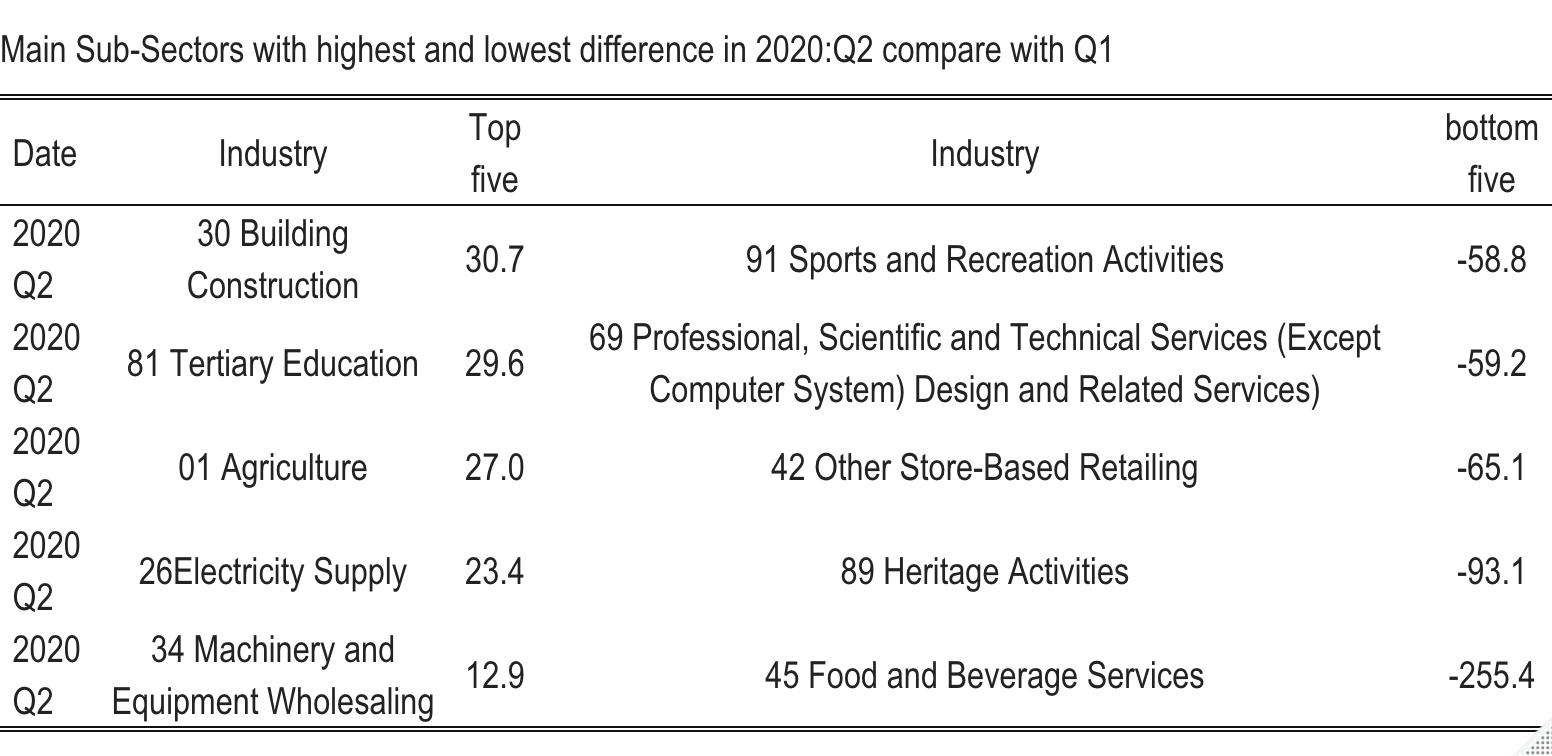
\includegraphics[scale=0.2]{Comparison}
\centering
\caption{The highest and lowest five sub-sectors' employment change in (10000) at 2020:Q2}
\label{fig:comp}
\end{figure}

\hypertarget{methdology}{%
\section{Methdology}\label{methdology}}

\hypertarget{proposed-model}{%
\subsection{Proposed Model}\label{proposed-model}}

I plan to use a Bayesian VARX model based on a method proposed by \textcite{anderson2020}. In the model, each sector is affected by the lags of sectoral growth and a lag of the total employment growth. The lag of aggregate employment growth act as an economy-wide factor which will affect each sector.

Under the assumption that the structure of Australian economy will not change during the COVID-19, we suggest the BVAR model as

\[
\begin{aligned}
\textbf{y}_t=\textbf{c}+\textbf{A}_1 \textbf{y}_{t-1}+\textbf{A}_2\textbf{y}_{t-2}+\textbf{A}_3\textbf{y}_{t-3}+\textbf{A}_4\textbf{y}_{t-4}+\bf{\Gamma}\textbf{x}_{t-1}+\bf{u}_t
\end{aligned}
\]

where \(\bf{y}_t\) is an \(87\times1\) vector of subsectoral employment growth rate at time \(t\) and \(\bf{x}_{t-1}\) is the \(4\times1\) vector of 4 lags of the growth rate of aggregate employment (this vector of variables are predetermined at time \(t\)), \textbf{c} is a vector of constants, \(\bf{A}_{1,2,3,4}\) are \(87\times87\) parameter matrices. \(\bf{\Gamma}\) is a \(87\times4\) matrix and \(\bf{u}_t\) is a vector of reduced form errors with the mean equals to zero and independent variance \(\bf{u}_t \sim (0,\bf{\Sigma})\). (see Appendix)

\hypertarget{prior-and-shrinkage}{%
\subsection{Prior and shrinkage}\label{prior-and-shrinkage}}

I plan to estimate the VARX using Bayesian methods by specifying a Minnesota prior \autocites[e.g.][]{anderson2020,litterman1986,robertson1999vector}. In order to set up the Minnesota prior in our BVAR model, \textcite{banbura2010large} suggestes a nature conjugate Normal-Wishart prior that applies shrinkage to the VAR slope coefficients using a Minnesota-type prior.

\[
\begin{aligned}
&E[a_{j}^{jk}] = E[\gamma_{i}^j]=0\\
\\
&Var[a_j^{jk}]= 
\begin{cases}
\frac{\lambda^2}{i^2},&j=k\\
\frac{\lambda^2}{i^2}\frac{\sigma^2_{j}}{\sigma^2_k},& otherwise
\end{cases}\\
\\
&Var[\gamma_i^{j}]=\frac{\lambda^2}{i^2}\frac{\sigma^2_{j}}{\sigma^2_e}
\end{aligned}
\]

\textcite{banbura2010large} stated that the natural conjugate Normal-Inverse-Wishart posterior moments can be calculated either analytically or though adding the dummy observations. I will use dummy observations to estimate the BVAR e.g.\autocite{banbura2010large,anderson2020,wozniak2016bayesian}. An example completed by \textcite{anderson2020} will be given in the Appendix. After the estimation of Bayesian VAR and then amounts to conducting least squares, we can draw our VAR coefficients by solving the posterior mode and mean.

\hypertarget{timeline-and-expected-outcome}{%
\section{Timeline and expected outcome}\label{timeline-and-expected-outcome}}

Table \ref{tab:timeline1} summarises the work done to date. Table \ref{tab:timeline2} maps out the plan for completing the thesis research.

It is expected that we will have an accurate multivariate BVAR model to forecast the scenario without COVID-19 based on the data of 87 sub-sectors before 2019. Then we have some

\begin{table}

\caption{\label{tab:timeline1}Completed work}
\centering
\begin{tabular}[t]{ll}
\toprule
Timeline & Tasks\\
\midrule
Week 2 & Background reading about Multivariate VAR model\\
Week 3 & Collect Sub-sectoral data from ABS website\\
 & Prepare materials reltaed to subsectoral employment evaluations\\
Week 4 & Prepare literature review related to BVAR model and setting priors\\
 & Analysis about the MATLAB code done by Andereson et al. (2020)\\
\addlinespace
Week 5 & Read articles about Conditional Forecasting\\
Week 6 & Prepare the conditional forecasting coding and hierarchical forecasting\\
Week 7 & Exploratory data analysis on sectoral and subsectoral data\\
Week 8 & Select suitable plots and test softwares to prepare the proposal\\
week 9 & Write research proposal and prepare the first presentation\\
\bottomrule
\end{tabular}
\end{table}

\begin{table}

\caption{\label{tab:timeline2}Research plan}
\centering
\begin{tabular}[t]{ll}
\toprule
Timeline & Tasks\\
\midrule
June - July & Modelling of subsectoral employment\\
August & Train the model using pre-covid data with BVAR model\\
September & apply foreecasts for quarters between 2020 to 2022\\
October & Write my thesis and prepare for the second presentation\\
\bottomrule
\end{tabular}
\end{table}

\newpage

\hypertarget{acknowledgement}{%
\section{Acknowledgement}\label{acknowledgement}}

I would like to gratitude my supervisor Professor Farshid Vahid and my coordinator Professor Heather Anderson very much for their selfless support and devoted care along the way.

\hypertarget{appendix}{%
\section{Appendix}\label{appendix}}

Here is an example of the BVAR estimation done by \textcite{anderson2020}.

\begin{align}
\textbf{y}_t&=\textbf{c}+\textbf{A}_1 \textbf{y}_{t-1}+\textbf{A}_2+\cdots+\textbf{A}_4\textbf{y}_{t-4}+\bf{\Gamma}_1\textbf{x}_{t-1}+\bf{u}_t\\
&=
\begin{bmatrix}
c_1\\
\vdots\\
c_2
\end{bmatrix}
+
\begin{bmatrix}
a_1^{11}&\cdots&a_1^{1n}&\cdots&a_4^{11}&\cdots&a_4^{1n}&\gamma_1^{1}&\cdots&\gamma_4^{1}\\
\vdots&\ddots&\vdots&\ddots&\vdots&\ddots&\vdots&\vdots&\ddots&\vdots\\
a_1^{n1}&\cdots&a_1^{nn}&\cdots&a_4^{n1}&\cdots&a_4^{nn}&\gamma_1^n&\cdots&\gamma_4^n\\
\end{bmatrix}
\begin{bmatrix}
\bf{y}_{t-1}\\
\vdots\\
\bf{y}_{t-4}\\
x_{t-1}\\
\vdots\\
x_{t-4}
\end{bmatrix}\\
&+
\begin{bmatrix}
u_{1,t}\\
\vdots\\
u_{n,t}
\end{bmatrix}\\
\end{align}

where \(E(\bf{u}_t\bf{u}'_t)=\bf{\Sigma}\) and \(E(\bf{u}_t\bf{u'}_{t-1})=0\). Here the \(n\) represent the number of sectors (or in our case will be 87) and \(c\)represents the vector of constants. There are 4 lags included for the total employment \((x_{t-1},\cdots,x_{t-4})\) as predetermined variable at time t.

Here is an Minnesota prior example done by \textcite{anderson2020}:

The Normal-Wishart prior distribution take the form of

\[
\begin{aligned}
&vec(\mathbf{\beta}|\Sigma)\sim N(vec(\bf{\beta_0}),\Sigma\otimes\Omega_0)\ and\\
&\Sigma\sim\mathbf{IW}(S_0,a_0)
\end{aligned}
\] where we set the prior parameters and \(a_0\) based on the prior setting. The expectation of \(\Sigma\) being \(diag(\sigma^2_1,\cdots,\sigma^2_n\). Then we implement our VAR by defining dummy observations

\[
\begin{aligned}
Y_d&=
\begin{pmatrix}
\bf0_{np+p,n}\\
\bf diag(\bf{\sigma_1,\cdots,\sigma_n})\\
\bf0_{1\times n}
\end{pmatrix}\\
X_d&=
\begin{pmatrix}
\bf{J_p}\otimes diag(\frac{\sigma_1}{\lambda}\cdots\frac{\sigma_n}{\lambda},\frac{\sigma_e}{\lambda})&\bf0_{(np+p)\times1}\\
\bf 0_{n,np+p}&\bf 0_{n\times1}
\\
\bf 0_{1,np+p}&\bf \epsilon
\end{pmatrix}
\end{aligned}
\] where

\[
\begin{aligned}
\bf{J_p}=diag(1,\cdots,p)\\
\bf{S_0}=(Y_d-X_d\times B_0)'(Y_d-X_dB_0)\\
\bf{B_0}=(X_d'X_d)^{-1}X_dY_d,\ \Omega_0=(X_d'X_d)^{-1}\  and\\
a_0=T_d-np-p-1\\
\end{aligned}
\] where \(T_d\) is the number of rows for both \(\bf{Y}_d\) and \(\bf{X}_d\).

We can get \[
\begin{aligned}
\bf{Y^*}=\bf{X^*}\bf{\beta}+\bf{\mu}^*\ \ \  where: \\
\bf{Y^*}=[\bf{Y'},\bf{Y'_d}]';\ \bf{X^*}=[\bf{X'},\bf{X'_d}]';\ \bf{\mu^*}=[\bf{\mu'},\bf{\mu'_d}]'
\end{aligned}
\]

Then we can estimating the BVAR by conducting an least square regression of \(Y^*\) on\(X^*\). The posterior distribution then have the form of

\[
\begin{aligned}
&vec(\mathbf{\beta})|\Sigma,Y\sim N(vec(\bf{\tilde\beta}),\Sigma\otimes(\bf{X^*}'\bf{X^*})^{-1})\ and\\
&\Sigma|Y\sim\mathbf{IW}(\tilde\Sigma,T_d+T-np+2)
\end{aligned}
\] where \(\bf{\tilde\beta} =(X*'X*)^{-1}X^{*'}Y^*\) and \(\tilde\Sigma=(\bf{Y^*}-\bf{X^*}\bf{\tilde\beta})'(\bf{Y^*}-\bf{X^*}\bf{\tilde\beta})\)

\newpage

\begin{figure}[t]
\includegraphics[scale=0.6]{free_19}
\centering
\caption{Employment('000) of 19 sectors in Australia from 2019:Q1 to 2021:Q4}
\label{fig:19}
\end{figure}

\begin{figure}[t]
\includegraphics[scale=0.5]{free_87}
\centering
\caption{Employment('000) of 87 sub-sectors in Australia from 2019:Q1 to 2021:Q4}
\label{fig:87}
\end{figure}

\begin{figure}[t]
\includegraphics[scale=0.5]{ANZSIC}
\centering
\caption{Australian Industry Pamamid plot by (ANZSIC)}
\label{fig:anzsic}
\end{figure}

\clearpage

\printbibliography

\end{document}
